\section{Математическая модель}
\label{sec:math_model}

В данном разделе описаны две модели. Математическая модель №1 является расширением модели, построенной в \cite{ivanov2014mccablockack}. Данная модель при расчёте учитывает распределение $\{ p_{ij} \}_{i=1, j=1}^{i=M, j=M}$ , где $p_{ij}$ --- вероятность того, что за пачкой размера $i$ будет передаваться пачка размера $j$. Однако, несмотря на использование этого распределения, с помощью Математической модели №1 не удастся выбрать параметры резервирования так, чтобы потребление канальных ресурсов было минимально.
Поэтому была построена Математическая модель №2, которая помимо этого распределения будет также учитывать состояние очереди поступивших на передачу пакетов, что оказывается важным при передаче мультимедийного потока в режиме реального времени.

%Новая модель по сравнению со старой является более сложной в смысле используемой информации. Если в старой модели формировалась цепь Маркова, учитывающая только распределение вероятностей размеров пачек, то в новой же используется распределение вероятностей размеров пачек при условии, какой размер имела предыдущая пачка.
%Данная модификация предположительно позволит добиться лучшей сходимости по сравнению с первоначальной моделью. И поскольку обе эти модели сходятся в предположении о стационарности описанных в ней состояний, на деле они расходятся, поскольку предположительно во время передачи мультимедийного потока время установления стационарного состояния сравнительно велико по сравнению с длительностью передачи потока.


\subsection{Математическая модель №1}
\label{subsec:mathmodel_1}

\subsubsection{Цепь Маркова}
\label{subsubsec:markovchain_1}
Представим $\Tin/\Tres$ в виде несократимой дроби $\tin/\tres$, где $\tin, \tres\in\mathbb{N}$. Назовем слотом интервал времени длины $$\tau \equiv  \frac{\Tin}{\tin} = \frac{\Tres}{\tres}.$$ Разобьем непрерывную временную шкалу на слоты таким образом, чтобы начало каждого зарезервированного интервала совпадало с началом некоторого слота -- см.~рис~\ref{fig:time}.

Процесс передачи пакетов с помощью механизма периодических резервирований может быть описан цепью Маркова с дискретным временем, единица которого равна периоду резервирований.

\begin{figure}[t]
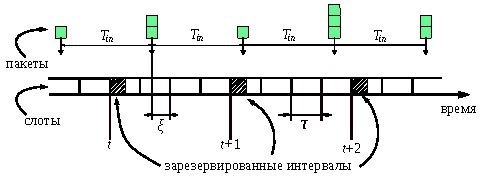
\includegraphics[width=\linewidth]{MarkChain.pdf}
\caption{\label{fig:time} Слотированное время}
\end{figure} 

В каждый момент времени $t$ состояние системы будем описывать парой целых чисел $(h(t), m(t), n(t))$. Если $h(t) \geqslant 0$, то очередь не пуста, и $h(t)$ равно числу полных слотов, которые головная (самая старшая) пачка пакетов провела в очереди, $m(t)$ равно числу пакетов в этой пачке, а $n(t)$ равно начальному числу пакетов в головной пачке. Если $h(t) < 0$, то очередь пуста, и $|h(t)|$ равно времени до прибытия новой пачки пакетов, выраженному в слотах и округленному вниз; при этом $m=n$, а $n$ задаётся случаным образом, исходя из распределения $\{ p_{ij} \}_{i=1, j=1}^{i=M, j=M}$ и начальным размером предыдущей головной пачки. Это значит, что в любой момент времени $m(t) > 0$. Таким образом, состояние системы в каждый моменты времени $t$ характеризуется текущим числом пакетов в головной пачке, начальным числом пакетов  в головной пачке и временем, в течение которого пакеты этой пачки ожидают передачи. Используемые обозначения состояния системы позволяют определить количество пачек пакетов в очереди, ($\lfloor h(t)/\tin \rfloor + 1$ в момент времени $t$), но не позволяют определить длины всех пачек, кроме головной. После того, как все пакеты головной пачки были переданы или отброшены, определяется число пакетов в пачке, ставшей головной.
  
Минимальное значение $h(t)$ равно $\tres-\tin$. Оно достигается в момент времени $t$, если пачка из одного пакета пребывает в пустую очередь непосредственно перед моментом $t - 1$, и единственный пакет пачки успешно передается с первой попытки.   

Теперь найдем максимальное возможное значение $h(t)$. Для этого обозначим через $\xi$ время между поступлением пачки пакетов в очередь и началом следующего слота, $0 \leqslant \xi < \tau$. В силу того, что время $\Tin$ равно целому числу $\tin$ слотов, значение величины $\xi$ одинаково для всех пачек. Таким образом, к моменту времени $t$ время ожидания в очереди пакетов головной пачки равно $h(t) \cdot \tau + \xi$. Чтобы эта пачка не была отброшена в момент $t$, ее время ожидания не должно превышать значения $D$. Следовательно, $h(t) \leqslant d = \lfloor \frac{D-\xi}{\tau} \rfloor$. 

Благодаря тому, что числа $\tin$ и $\tres$ взаимно просты, цепь Маркова обладает свойством эргодичности. Таким образом, может быть найдено стационарное распределение вероятностей цепи Маркова. 

Выясним, в какие состояния и с какой вероятностью может перейти система из состояния $(h, m, n)$ за один шаг. Для этого отдельно рассмотрим несколько случаев.

\paragraph{1.} Пусть $h < 0$. Тогда на данный момент очередь пуста, значит, система перейдёт в состояние $(h + \tres, m, m)$.

\paragraph{2.} Пусть $d - \tres< h$. Тогда очередь не пуста, но к моменту начала следующего интервала резервирования истечёт время $\DQoS$ ожидания пакетов в головной пачке к моменту времени $t + 1$ система окажется в состоянии $(h + \tres - \tin, i, i)$ с вероятностью $p_{ni}$. Однако, следует учесть, что в этом случае с вероятностью $\qdet p_{ni}$ было потеряно $m$ пакетов, поскольку попытка передачи была неуспешной, а с вероятностью $(1 - \qdet) p_{ni}$ --- $m - 1$ , $i \in \{ 1, \ldots, M \}$. 

\paragraph{3.} Пусть $0 \leq h \leq d - \tres$. Тогда очередь не пуста, и к моменту времени $t + 1$ система окажется в состоянии:
\begin{itemize}
\item $(h + \tres, m, n)$ с вероятностью $\qdet$ в случае неудачной попытки передачи.
\item в случае удачной попытки передачи:
	\begin{itemize}
	\item $(h - \tin + \tres, i, i)$ с вероятностью $(1 - \qdet)p_{ni}$, если $m(t) = 1$;		
	\item $(h + \tres, m - 1, n)$ с вероятностью $(1 - \qdet)$, если  $m(t) > 1$.
	\end{itemize}
\end{itemize}

\paragraph{Подводя итог,} получаем, что при выполнении соответствующих условий система  переходит из состояния $(h, m, n)$ в одно из следующих состояний:

\begin{tabular}{l l l l}
1)	&$(h + \tres, m, m)$,	&$\gamma = 1$,	&при $h < 0$;\\
2)	&$(h + \tres - \tin, i, i)$,	&$\gamma = p_{ni}$,	&при $d - \tres< h$;\\
3)	&$(h + \tres, m, n)$,	&$\gamma = \qdet$,	&при $0 \leq h \leq d - \tres$;\\
4)	&$(h - \tin + \tres, i, i)$,	&$\gamma = ( 1 - \qdet) p_{ni}$,	&при $m = 1$, $0 \leq h \leq d - \tres$;\\
5)	&$(h + \tres, m - 1, n)$,	&$\gamma = ( 1 - \qdet)$,	&при $m > 1$, $0 \leq h \leq d - \tres$;\\
\end{tabular} \newline
где $i\in\{1,\ldots,M\}$ и $\gamma$ --- вероятность перехода. 

\subsubsection{Определение PLR}
Упорядочив состояния в лексикографическом порядке и построив матрицу $P$ переходных вероятностей, найдем стационарные вероятности $\pi_{(h,m,n)}$ состояний $(h,m,n)$.

Зная станционарные вероятности $\pi_{(h,m, n)}$, найдем долю $PLR$ потерянных пакетов. Так как пакеты отбрасываются только при превышении порога времени $\DQoS$ ожидания в очереди, потери пакетов могут происходить только при переходе $2$. Как упоминалось ранее, в случае успешной попытки передачи будет потерян $m - 1$ пакет, в ином случае --- $m$ пакетов. Тогда среднее число пакетов, отбрасываемых за один шаг модельного времени ($\Tres$), равно
$$
	\Idis = \sum\limits_{(h,m, n)\colon h > d - \tres} \left((m - 1)(1 - \qdet)\pi_{(h,m,n)} + m\qdet\pi_{(h,m,n)}\right) = \\
	=\sum\limits_{(h,m,n)\colon h > d - \tres} (m - 1 + \qdet)\pi_{(h,m,n)}.
$$

Значение $PLR$ равно отношению среднего числа $\Idis$ пакетов, отброшенных за один шаг модельного времени, к среднему числу $\Iin$ пакетов, поступивших в очередь за то же время:
$$
PLR = \frac{\Idis}{\Iin} = \frac{1}{\frac{\Tres}{\Tin} \sum\limits_{i} i\cdot p_i} \cdot \left(\sum\limits_{(h,m,n)\colon h > d - \tres} (m - 1 + \qdet)\pi_{(h,m,n)} \right).
$$
\subsection{Математическая модель №2}
\label{subsec:mathmodel_2}

Данная модель в общем случае рассматривает процесс передачи пакетов в случае известной очереди пакетов в начальный момент времени. Данное обстоятельство не использовалась в предыдущей модели, однако знание о текущей очереди может помочь подобрать наиболее подходящий период резервирования.

Идея этой модели основана на том, что в моменты времени, когда изначальная очередь не пуста, происходят однозначные переходы относительно размера следующей пачки. Когда очередь становится пустой, протекают всевозможные переходы по всем размерам следущей пачки.

Состояние системы описывается той же тройкой параметров, что и в \ref{subsec:mathmodel_1}. В каждый момент времени каждому состоянию $(h, m, n)$ будет соответствовать:
\begin{itemize}
\item его вероятность $\pi_{(h, m, n)}$;
\item среднее число потерянных пакетов по прибытию в данное состояние $\lost_{(h, m, n)}$;
\item среднее число \textit{обработанных} пакетов $\proc_{(h, m, n)}$, т.е. таких пакетов, которые по прибытию в данное состояние были либо успешно доставлены, либо отброшены. Это определение далее поможет в корректном вычислении $PLR$ в случае частично известного передаваемого потока.
\end{itemize}

Назовём \textit{фронтом состояний} системы в момент времени $t$ множество всех возможных состояний $(h(t), m(t), n(t))$, в которые система может попасть с ненулевой вероятностью. Будем рассматривать систему в моменты начал интервалов резервирования, в каждом из которых она имеет свой фронт $F(t)$.
%Будем считать, что если моменты резервирования и поступления пачки происходят в одно и то же время, то момент поступления пачки наступает раньше начала резервирования.

\subsubsection{Цепь Маркова в случае неизвестного передаваемого потока}
\label{subsec:mathmodel_2_unknown}

Будем считать известной матрицу переходных вероятностей $\{ p_{ij} \}_{i=1, j=1}^{i=M, j=M}$, а также распределение вероятностей размеров пачек $\{ p_i \}_{i=1}^{i=M}$.

Начнём рассматривать систему в момент наступления первого резервирования. Тогда начальный фронт будет состоять из состояний $(\xi, i, i)$, $i \in \{ 1, \ldots, M \}$, $\pi_{(\xi, i, i)} = p_i$, $\lost_{(\xi, i, i)} = \proc_{(\xi, i, i)} = 0$. Такая цепь Маркова ничем не отличается от цепи Маркова в \ref{subsec:mathmodel_1}, однако необходимо определить, сколько в среднем будет потеряно и обработано пакетов в каждом переходе. Таким образом, система  переходит из состояния $(h, m, n)$ в одно из следующих состояний:

\begin{tabular}{l l l l}
\label{mathmodel2_tab}
1)	&$(h + \tres, m, m)$,	&$\gamma = 1$,	&при $h < 0$,\\
	&$\Delta\lost = 0$,		&$\Delta\proc = 0$;\\
2)	&$(h + \tres - \tin, i, i)$,	&$\gamma = p_{ni}$,	&при $d - \tres< h$,\\
	&$\Delta\lost = m - 1 + \qdet$,	&$\Delta\proc = m$;\\
3)	&$(h + \tres, m, n)$,	&$\gamma = \qdet$,	&при $0 \leq h \leq d - \tres$,\\
	&$\Delta\lost = 0$,		&$\Delta\proc = 0$;\\
4)	&$(h - \tin + \tres, i, i)$,	&$\gamma = ( 1 - \qdet) p_{ni}$,	&при $m = 1$, $0 \leq h \leq d - \tres$,\\
	&$\Delta\lost = 0$,		&$\Delta\proc = 1$;\\
5)	&$(h + \tres, m - 1, n)$,	&$\gamma = ( 1 - \qdet)$,	&при $m > 1$, $0 \leq h \leq d - \tres$;\\
	&$\Delta\lost = 0$,		&$\Delta\proc = 1$;\\
%\caption{Таблица переходных вероятностей в цепи Маркова математической модели №2 в случае низвестного передаваемого потока}
\end{tabular} \newline
где $i\in\{1,\ldots,M\}$, $\gamma$ --- вероятность перехода, 	$\Delta\lost$, $\Delta\proc$ --- среднее число отброшенных и обработанных пакетов за переход соответственно.

%Тогда единственным отличием между переходами из состояний в фронте $F_i$  в состояния в фронте $F_{i+1}$ в цепи Маркова в случае неизвестного передаваемого потока и в случае заранее известного передаваемого потока является то, что переходы, где $n$ переходит в $n+1$ в случае заданного потока, в случае неизвестного потока $n$ переходит в $i$, а $m$ переходит в $i$ с вероятностью $p_{ni}$, $i \in \{ 1, \ldots, M \}$.

\subsubsection{Цепь Маркова в случае заранее известного передаваемого потока}
\label{subsec:mathmodel_2_know}

В данном случае рассмотрим передачу пакетов следующим образом. Будем считать, что размеры пачек входного потока  заранее известны, т.е. наперед известен размер $\flowsize$ потока $\flow$ в пачках и размер каждой из них $\flow_i, i = \overline{1, \flowsize}$ в пакетах. Состояние системы будет описываться той же тройкой параметров $(h,m,n)$, что и в \ref{subsec:mathmodel_2_unknown}, с той лишь поправкой, что $n$ равно номеру старшей пачки в потоке. Следовательно, $1 \leq n \leq \flowsize$.

В начальный момент времени система находится в состоянии $(\xi, B_1, 1)$. Переходы из фронта $F(t)$ в фронт $F(t+1)$ описываются \ref{mathmodel2_tab}, однако в ней надо учесть то, что поток заранее известен. Таким образом, получим следующие переходы из состояния $(h, m, n)$:

\begin{tabular}{l l l l}
\label{mathmodel2_tab_know}
1)	&$(h + \tres, m, n)$,	&$\gamma = 1$,	&при $h < 0$,\\
	&$\Delta\lost = 0$,		&$\Delta\proc = 0$;\\
2)	&$(h + \tres - \tin, \flow_{n+1}, n + 1)$,		&$\gamma = 1$,	&при $d - \tres< h$, $n < \flowsize$\\
	&$\Delta\lost = m - 1 + \qdet$,	&$\Delta\proc = m$;\\
3)	&$(h + \tres, m, n)$,	&$\gamma = \qdet$,	&при $0 \leq h \leq d - \tres$,\\
	&$\Delta\lost = 0$,		&$\Delta\proc = 0$;\\
4)	&$(h - \tin + \tres, \flow_{n+1}, n+1)$,		&$\gamma = ( 1 - \qdet)$,	&при $m = 1$, $0 \leq h \leq d - \tres$, $n < \flowsize$\\
	&$\Delta\lost = 0$,		&$\Delta\proc = 1$;\\
5)	&$(h + \tres, m - 1, n)$,	&$\gamma = ( 1 - \qdet)$,	&при $m > 1$, $0 \leq h \leq d - \tres$;\\
	&$\Delta\lost = 0$,		&$\Delta\proc = 1$;\\
%\caption{Таблица переходных вероятностей в цепи Маркова математической модели №2 в случае низвестного передаваемого потока}
\end{tabular} \newline
где $i\in\{1,\ldots,M\}$, $\gamma$ --- вероятность перехода, 	$\Delta\lost$, $\Delta\proc$ --- среднее число отброшенных и обработанных пакетов за переход соответственно. В дополнение, все переходы имеют место при условии, что новое состояние $(h,m,n)$ имеет $n \leq \flowsize$.

%Рассмотрим возможные переходы из состояния $(h, m, n)$ в фронте $F_i$ $i$-ого резервирования в состояния в фронте $F_{i + 1}$ $(i+1)$-ого резервирования, а также прирост среднего числа потерянных пакетов за эти переходы. Также для каждого состояния будем находить прирост количества за переход \textit{обработанных} пакетов, т.е. тех пакетов, которые либо переданы, либо отброшены.

%\paragraph{1.} $h < 0$, т.~е. очередь пуста.
%
%\begin{itemize}
%\item Если $h + \Tres \geq 0$, то к моменту времени $t + 1$ в очередь поступит очередная пачка пакетов. Размер пачки заранее определён, поэтому с вероятностью $1$ система окажется в состоянии $(h + \Tres, B_{i+1}, i+1)$.
%
%\item Если же $h + \Tres < 0$, то к моменту времени $t + 1$ в очередь не поступит ни одного пакета, т.~е. в этом случае система с вероятностью $1$ перейдет в состояние $(h + \Tres, 0, i)$. 
%\end{itemize}
%
%В обоих случаях среднее число потерянных пакетов и число обработанных пакетов за переход равно нулю. 
%%%%W%%%%%%%%%%%%
%\paragraph{2.} Пусть $D \geq h(t) \geq 0$ и $m(t) = 1$, т.~е. в головной пачке находится единственный пакет.
%
%С вероятностью $1 - \qdet$ происходит успешная передача пакета.
%
%\begin{itemize}
%\item Если при этом $h - \Tin + \Tres < 0$, то к моменту времени $t + 1$ на станцию не поступит ни одной пачки данных и система окажется в состоянии $(h - \Tin + \Tres, 0, n)$ с вероятностью $1 - \qdet$.
%\item Если же $h - \Tin + \Tres \geqslant 0$, то в момент времени $t + 1$ очередь будет не пуста, и состояние системы будет определяться числом пакетов в головной пачке с номером  $n + 1$, тогда система перейдет в состояние $(h - \Tin + \Tres, B_{n+1}, n+1)$ с вероятностью $1 - \qdet$.
%\end{itemize}
%
%В обоих этих случаях среднее число потерянных пакетов за переход равно нулю. Число обработанных пакетов равно 1.
%
%С вероятностью $\qdet$ происходит неуспешная передача пакета.
%
%\begin{itemize}
%\item Если $h + \Tres > D$, то к моменту времени $t + 1$ время жизни данного пакета  превысит допустимое значение $D$, и этот пакет будет отброшен. Cистема c вероятностью $\qdet$ перейдет в состояние $(h - \Tin + \Tres, B_{n+1}, n + 1)$. Среднее число потерянных пакетов в этом переходе равно $\qdet$. Число обработанных пакетов равно 1.
%\item Если $h + \Tres \leq D$, то к моменту времени $t + 1$ пакет не устареет, и будет предпринята следующая попытка передачи. Следовательно, система перейдет в состояние $(h + \Tres, 1, n)$ с вероятностью $\qdet$. Среднее число потерянных пакетов в этом переходе равно нулю. Число обработанных пакетов равно нулю.
%\end{itemize}
%
%\paragraph{3.} Наконец, рассмотрим случай, когда $h(t) \geq 0$, $m(t) > 1$. 
%
%\begin{itemize}
%\item Если $h + \Tres > D$, то к моменту времени $t + 1$ время ожидания этих пакетов превысит допустимое значение $D$, и все пакеты пачки будут отброшены. Система с вероятностью $1$ перейдет в состояние $(h - \Tin + \Tres, B_{n+1}, n+1)$. Здесь среднее число потерянных пакетов за переход равно $m - 1 + \qdet$. Число обработанных пакетов равно $m$.
%\item Если $h + \Tres \leq D$, то система с вероятностью $1 - \qdet$ перейдет в состояние $(h + \Tres, m - 1, n)$, где число обработанных пакетов равно 1, а с вероятностью $\qdet$ перейдёт в состояние $(h + \Tres, m, n)$, где число обработанных пакетов равно нулю.
%\end{itemize}
%
%Здесь в обоих переходах среднее число потерянных пакетов равно нулю.
%
%После описания всевозможных переходов из фронта $F_i$ в фронт $F_{i+1}$ необходимо отнормировать все вероятности (в следующий фронт цепь попадает с вероятностью 1).
%
%\paragraph{Подводя итог,} получаем, что при выполнении соответствующих условий система  переходит из состояния $(h, m, n)$ в одно из следующих состояний:
%
%\begin{tabular}{l l l l l}
%1)	&$(h + \Tres, 0, n)$, 			&$\gamma = 1$, &$\Delta N_{lost} = 0$,	&при $m = 0$, $h < -\Tres$; \\
%2)  &$(h + \Tres, B_{n+1}, n+1)$, 			&$\gamma = 1$, &$\Delta N_{lost} = 0$, &при $m = 0$, $-\Tres \leqslant h < 0$; \\
%3)  &$(h + \Tres - \Tin, B_{n+1}, n+1)$, 	&$\gamma = 1 - \qdet$,  &$\Delta N_{lost} = 0$, &при $m = 1$, $\Tin - \Tres \leqslant h \leqslant D$; \\
%4)  &$(h + \Tres - \Tin, 0, n)$, 	&$\gamma = 1 - \qdet$,  &$\Delta N_{lost} = 0$, &при $m = 1$, $0 \leqslant h < \Tin - \Tres$; \\
%5)  &$(h + \Tres - \Tin, B_{n+1}, n + 1)$, 	&$\gamma = \qdet$,  &$\Delta N_{lost} = \qdet$, &при $m = 1$, $d - \Tres < h \leqslant D$; \\
%6)  &$(h + \Tres, m, n)$, 			&$\gamma = \qdet$,  &$\Delta N_{lost} = 0$, &при $m > 0$, $0 \leqslant h \leqslant D - \Tres$; \\
%7)  &$(h + \Tres - \Tin, B_{n+1}, n+1)$,	&$\gamma = 1$,  &$\Delta N_{lost} = m - 1 + \qdet$, &при $m > 1$, $d - \Tres < h \leqslant D$; \\
%8)  &$(h + \Tres, m - 1, n)$, &$\gamma = 1 - \qdet$,  &$\Delta N_{lost} = 0$, &при $m > 1$, $0 \leqslant h \leqslant D - \Tres$;
%\end{tabular} \newline
%где $\gamma$ --- вероятность перехода,  $\Delta N_{lost}$ --- среднее число потерянных пакетов за переход.

\subsubsection{Цепь Маркова в случае частично известного передаваемого потока}
\label{subsec:mathmodel_2_mixed}

Можно объединить две вышеописанные цепи Маркова, объединив в том числе начальные условия: пусть имеется известный входной поток $\flow$ размера $\flowsize$, распределение вероятностей размеров пачек $\{ p_i \}_{i=1}^{i=M}$, матрица переходных вероятностей $\{ p_{ij} \}_{i=1, j=1}^{i=M, j=M}$.
%, введя новый параметр $r$, являющийся индикатором об известности входного потока: если $r$ = 0, то поток в данном состоянии известен, иначе $r$ = 1.

Состояние описывается тройкой параметров $(h, m, n)$.
%$r$ --- вышеописанный индикатор об известности входного потока,
$h$ --- возраст головной пачки, $m$ --- количество оставшихся пакетов в головной пачке, а $n$ --- номер головной пачки, если $n \leq \flowsize$, в противном случае это начальный размер головной пачки.

В данной модели начальный фронт $F(0)$ содержит только одно начальное состояние $(\xi, \flow_1, 1)$. Далее, до тех пор, пока $n \leq l$, все переходы описываются так же, как и в \ref{subsec:mathmodel_2_know}. Но в случаях, когда по логике модели \ref{subsec:mathmodel_2_know}, значение $n$ должно быть равным $\flowsize + 1$, вместо этого состояние $(h, m, \flowsize)$ перейдёт в состояние $(h + \Tres - \Tin, i, i)$ с вероятностью $p_{\flow_\flowsize i}$, $i \in \{ 1, \ldots, M \}$. При этом среднее число потерянных пакетов за переход будет равно 0, если $m = 0$, или $m - 1 + \qdet$, если $m \geq 1$.
Далее происходят переходы, описанные в \ref{subsec:mathmodel_2_unknown}.

\subsubsection{Определение PLR}

Описав всевозможные переходы из состояний фронта $F(t)$ в состояния фронта $F(t+1)$, необходимо вычислить $\pi_{(h, m, n)}$, $\lost_{(h, m, n)}$, $\proc_{(h, m, n)}$ для каждого $(h, m, n) \in F(t+1)$.

Сначала вычисляются $\pi_{(h, m, n)}$:

\begin{equation*}
\pi_{(h, m, n)} = \sum\limits_{(h', m', n') \in F(t)} \pi_{(h', m', n')} p\left( (h', m', n') \to (h, m, n) \right),
\end{equation*}
где $p\left( (h', m', n') \to (h, m, n) \right)$ --- переходная вероятность из состояния $(h', m', n')$ в состояние $(h, m, n)$, каждая из которых описана в \ref{mathmodel2_tab}. После вычисления всех вероятностей их необходимо отнормировать (система перейдёт в одно из состояний следующего фронта с вероятностью 1).

Далее вычисляются $\lost_{(h, m, n)}$ и $\proc_{(h, m, n)}$:

\begin{equation*}
\lost_{(h, m, n)} = \sum\limits_{(h', m', n') \in F(t)} \pi_{(h', m', n')} p\left( (h', m', n') \to (h, m, n) \right) \cdot (\Delta\lost_{(h', m', n') \to (h, m, n)} + \lost_{(h', m', n')});
\end{equation*}
\begin{equation*}
\proc_{(h, m, n)} = \sum\limits_{(h', m', n') \in F(t)} \pi_{(h', m', n')} p\left( (h', m', n') \to (h, m, n) \right) \cdot (\Delta\proc_{(h', m', n') \to (h, m, n)} + \proc_{(h', m', n')}).
\end{equation*}

Будем рассматривать передачу только в течение временного промежутка $W$. Следовательно, в цепи Маркова нужно совершить переходы до фронта в момент времени:
$$
t_{stop} = \floor*{\frac{W - \xi}{\Tres} + 1},
$$
который есть номер первого резервирования при условии, что это резервирование выходит за пределы окна $W$.

Зная всевозможные состояния в последнем фронте $F(t_{stop})$ и соответствующее каждому из них среднее число отброшенных пакетов $\lost_{(h, m, n)}$ и число обработанных пакетов $\proc_{( h, m, n)}$, можно вычислить среднее число отброшенных пакетов к моменту наступления фронта $F(t_{stop})$:
$$
PLR = \sum\limits_{(h,m,n) \in F(t_{stop})} \pi_{(h,m,n)} \cdot \frac{\lost_{(h, m, n)}}{\proc_{(h, m, n)}}.
$$

С помощью вышеописанной модели можно найти параметры резервирования таким образом, чтобы удовлетворять QoS-требованиям.
%\input{plr_new}
%\input{channel}

